\chapter{Appendix A, Writing Systems}
\label{ch:appendixa}

\section{Writing systems}

\subsection{Alfabet fonetyczny \emph{chiwo}}

Alfabet fonetyczny ma 27 znaków i nie rozróżnia wielkości znaków.

\emph{chiwo} w wersji odręcznej, może wyglądać w następujący sposób:

\begin{center}
  
\includegraphics[width=5cm]{katia-signature.png}
\end{center}

Jest to odręczny zapis imienia \emph{Katia}, ręką samej cesarzowej,
\textbf{Katii mal Arkai}. Jej mąż, \textbf{So'tak mal Valor}, podpisuje się
następująco:

\begin{center}
  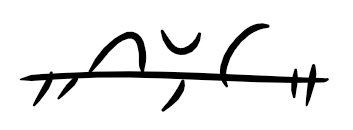
\includegraphics[width=5cm]{sotak.png}
\end{center}

Zapis w alfabecie fonetycznym, z wykorzystaniem specjalnego kroju \emph{desaho},
przeznaczonego do pisania znaków drogowych, informacji turystycznej i innych
informacji publicznych wygląda następująco:

\begin{center}
  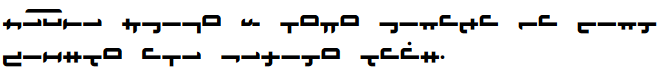
\includegraphics[width=12cm]{desaho.png}
\end{center}

\note{Tekst ten, \emph{ze͞uye chido yi boso hinaja va fint wirklo abe gepito laák}
  nie ma większego sensu, ale jest to pangram -- używany jako odpowiednik
  polskiego ,,pchnąć w tę łódź jeża lub ośm skrzyń fig''.}
\skipline

Ten sam tekst z wykorzystaniem popularnego kroju wzorowanego na piśmie
odręcznym, Na͞epo:

\begin{center}
  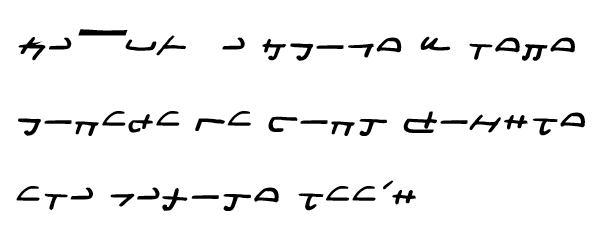
\includegraphics[width=12cm]{naepo.png}
\end{center}

\section{More on romanization}
\subsection{History}
\subsection{Conventions - punctuation and stress}

\section{Native script examples}